\documentclass{article}[11pt]
%Required: You must have these
\usepackage{graphicx}
\usepackage{tabularx}
\usepackage{natbib}

\usepackage{array}
\usepackage{amsmath}
%\usepackage[backend=bibtex]{biblatex}
\setkeys{Gin}{width=0.8\textwidth}
%\setlength{\captionmargin}{30pt}
\setlength{\abovecaptionskip}{10pt}
\setlength{\belowcaptionskip}{10pt}
\topmargin -1.5cm 
\oddsidemargin -0.04cm 
\evensidemargin -0.04cm 
\textwidth 16.59cm
\textheight 23.94cm 
\parskip 7.2pt 
\renewcommand{\baselinestretch}{1} 	
\parindent 0pt


\bibliographystyle{..//refs/styles/besjournals.bst}
\renewcommand{\thetable}{S\arabic{table}}
\renewcommand{\thefigure}{S\arabic{figure}}
%\usepackage{xr}
%\usepackage{hyperref}
\usepackage{xr-hyper}
\usepackage{hyperref}
\externaldocument{plum_manuscript}


\title{Supporting Information for: Ecological drivers of flower-leaf sequences: aridity and pollination success select for flowering-first in The American Plums} %emw: check title if you change it
\date{}
\usepackage{Sweave}
\begin{document}
\input{suppliment-concordance}
\maketitle

\section*{Tables}
\begin{table}[ht]
\centering
\begin{tabular}{rlrrr}
  \hline
 & species & n.FLS & n.petal & n.pdsi \\ 
  \hline
1 & alleghaniensis &  17 &  39 & 114 \\ 
  2 & americana &  95 & 271 & 200 \\ 
  3 & angustifolia &  77 & 238 & 200 \\ 
  4 & gracilis &  85 & 289 & 200 \\ 
  5 & hortulana & 106 & 254 & 200 \\ 
  6 & maritima &  75 & 255 & 200 \\ 
  7 & mexicana &  64 & 284 & 200 \\ 
  8 & munsoniana & 117 & 279 & 200 \\ 
  9 & nigra & 118 & 230 & 200 \\ 
  10 & rivularis & 111 & 225 & 200 \\ 
  11 & subcordata &  46 &  71 &  30 \\ 
  12 & texana &  19 &  38 &  39 \\ 
  13 & umbellata &  70 & 284 & 200 \\ 
   \hline
\end{tabular}
\caption{Sample sizes of each for each species used in this study}
\label{tab:samps}
\end{table}

% latex table generated in R 4.1.2 by xtable 1.8-4 package
% Mon Oct  2 18:15:48 2023
\begin{table}[ht]
\centering
\begin{tabular}{rlrr}
  \hline
 & species & index & index.nodoy \\ 
  \hline
1 & mexicana & 0.85 & 0.90 \\ 
  2 & umbellata & 0.82 & 0.83 \\ 
  3 & angustifolia & 0.76 & 0.77 \\ 
  4 & maritima & 0.68 & 0.76 \\ 
  5 & gracilis & 0.64 & 0.68 \\ 
  6 & americana & 0.62 & 0.55 \\ 
  7 & munsoniana & 0.60 & 0.67 \\ 
  8 & alleghaniensis & 0.59 & 0.65 \\ 
  9 & nigra & 0.55 & 0.62 \\ 
  10 & hortulana & 0.51 & 0.52 \\ 
  11 & texana & 0.51 & 0.54 \\ 
  12 & rivularis & 0.44 & 0.53 \\ 
  13 & subcordata & 0.16 & 0.18 \\ 
   \hline
\end{tabular}
\end{table}

% xtable(fixef(mod.review.wants,probs = c(.055,.25,.75,.945)))
% latex table generated in R 4.1.2 by xtable 1.8-4 package
% Mon Oct  2 16:33:58 2023
\begin{table}[ht]
\centering
\begin{tabular}{rrrrrrr}
  \hline
 & Estimate & Est.Error & Q5.5 & Q25 & Q75 & Q94.5 \\ 
  \hline
Intercept & 0.34 & 0.23 & -0.02 & 0.20 & 0.48 & 0.70 \\ 
  phi\_Intercept & 1.92 & 0.42 & 1.22 & 1.65 & 2.21 & 2.55 \\ 
  pdsi.z & -0.47 & 0.30 & -0.96 & -0.66 & -0.28 & 0.01 \\ 
  petal.z & -0.14 & 0.24 & -0.54 & -0.29 & 0.01 & 0.23 \\ 
  pdsi.z:petal.z & -0.14 & 0.49 & -0.91 & -0.46 & 0.16 & 0.65 \\ 
   \hline
\end{tabular}
\end{table}
% xtable(fixef(mod.review.wants.doy,probs = c(.055,.25,.75,.945)))
% latex table generated in R 4.1.2 by xtable 1.8-4 package
% Mon Oct  2 16:34:12 2023
\begin{table}[ht]
\centering
\begin{tabular}{rrrrrrr}
  \hline
 & Estimate & Est.Error & Q5.5 & Q25 & Q75 & Q94.5 \\ 
  \hline
Intercept & 0.49 & 0.25 & 0.09 & 0.33 & 0.65 & 0.88 \\ 
  phi\_Intercept & 1.77 & 0.41 & 1.09 & 1.50 & 2.06 & 2.39 \\ 
  pdsi.z & -0.43 & 0.32 & -0.92 & -0.63 & -0.22 & 0.07 \\ 
  petal.z & -0.14 & 0.27 & -0.56 & -0.30 & 0.03 & 0.27 \\ 
  pdsi.z:petal.z & -0.16 & 0.54 & -1.01 & -0.50 & 0.17 & 0.69 \\ 
   \hline
\end{tabular}
\end{table}
\pagebreak

\section*{Figures} 
\begin{figure}[h!]
    \centering
 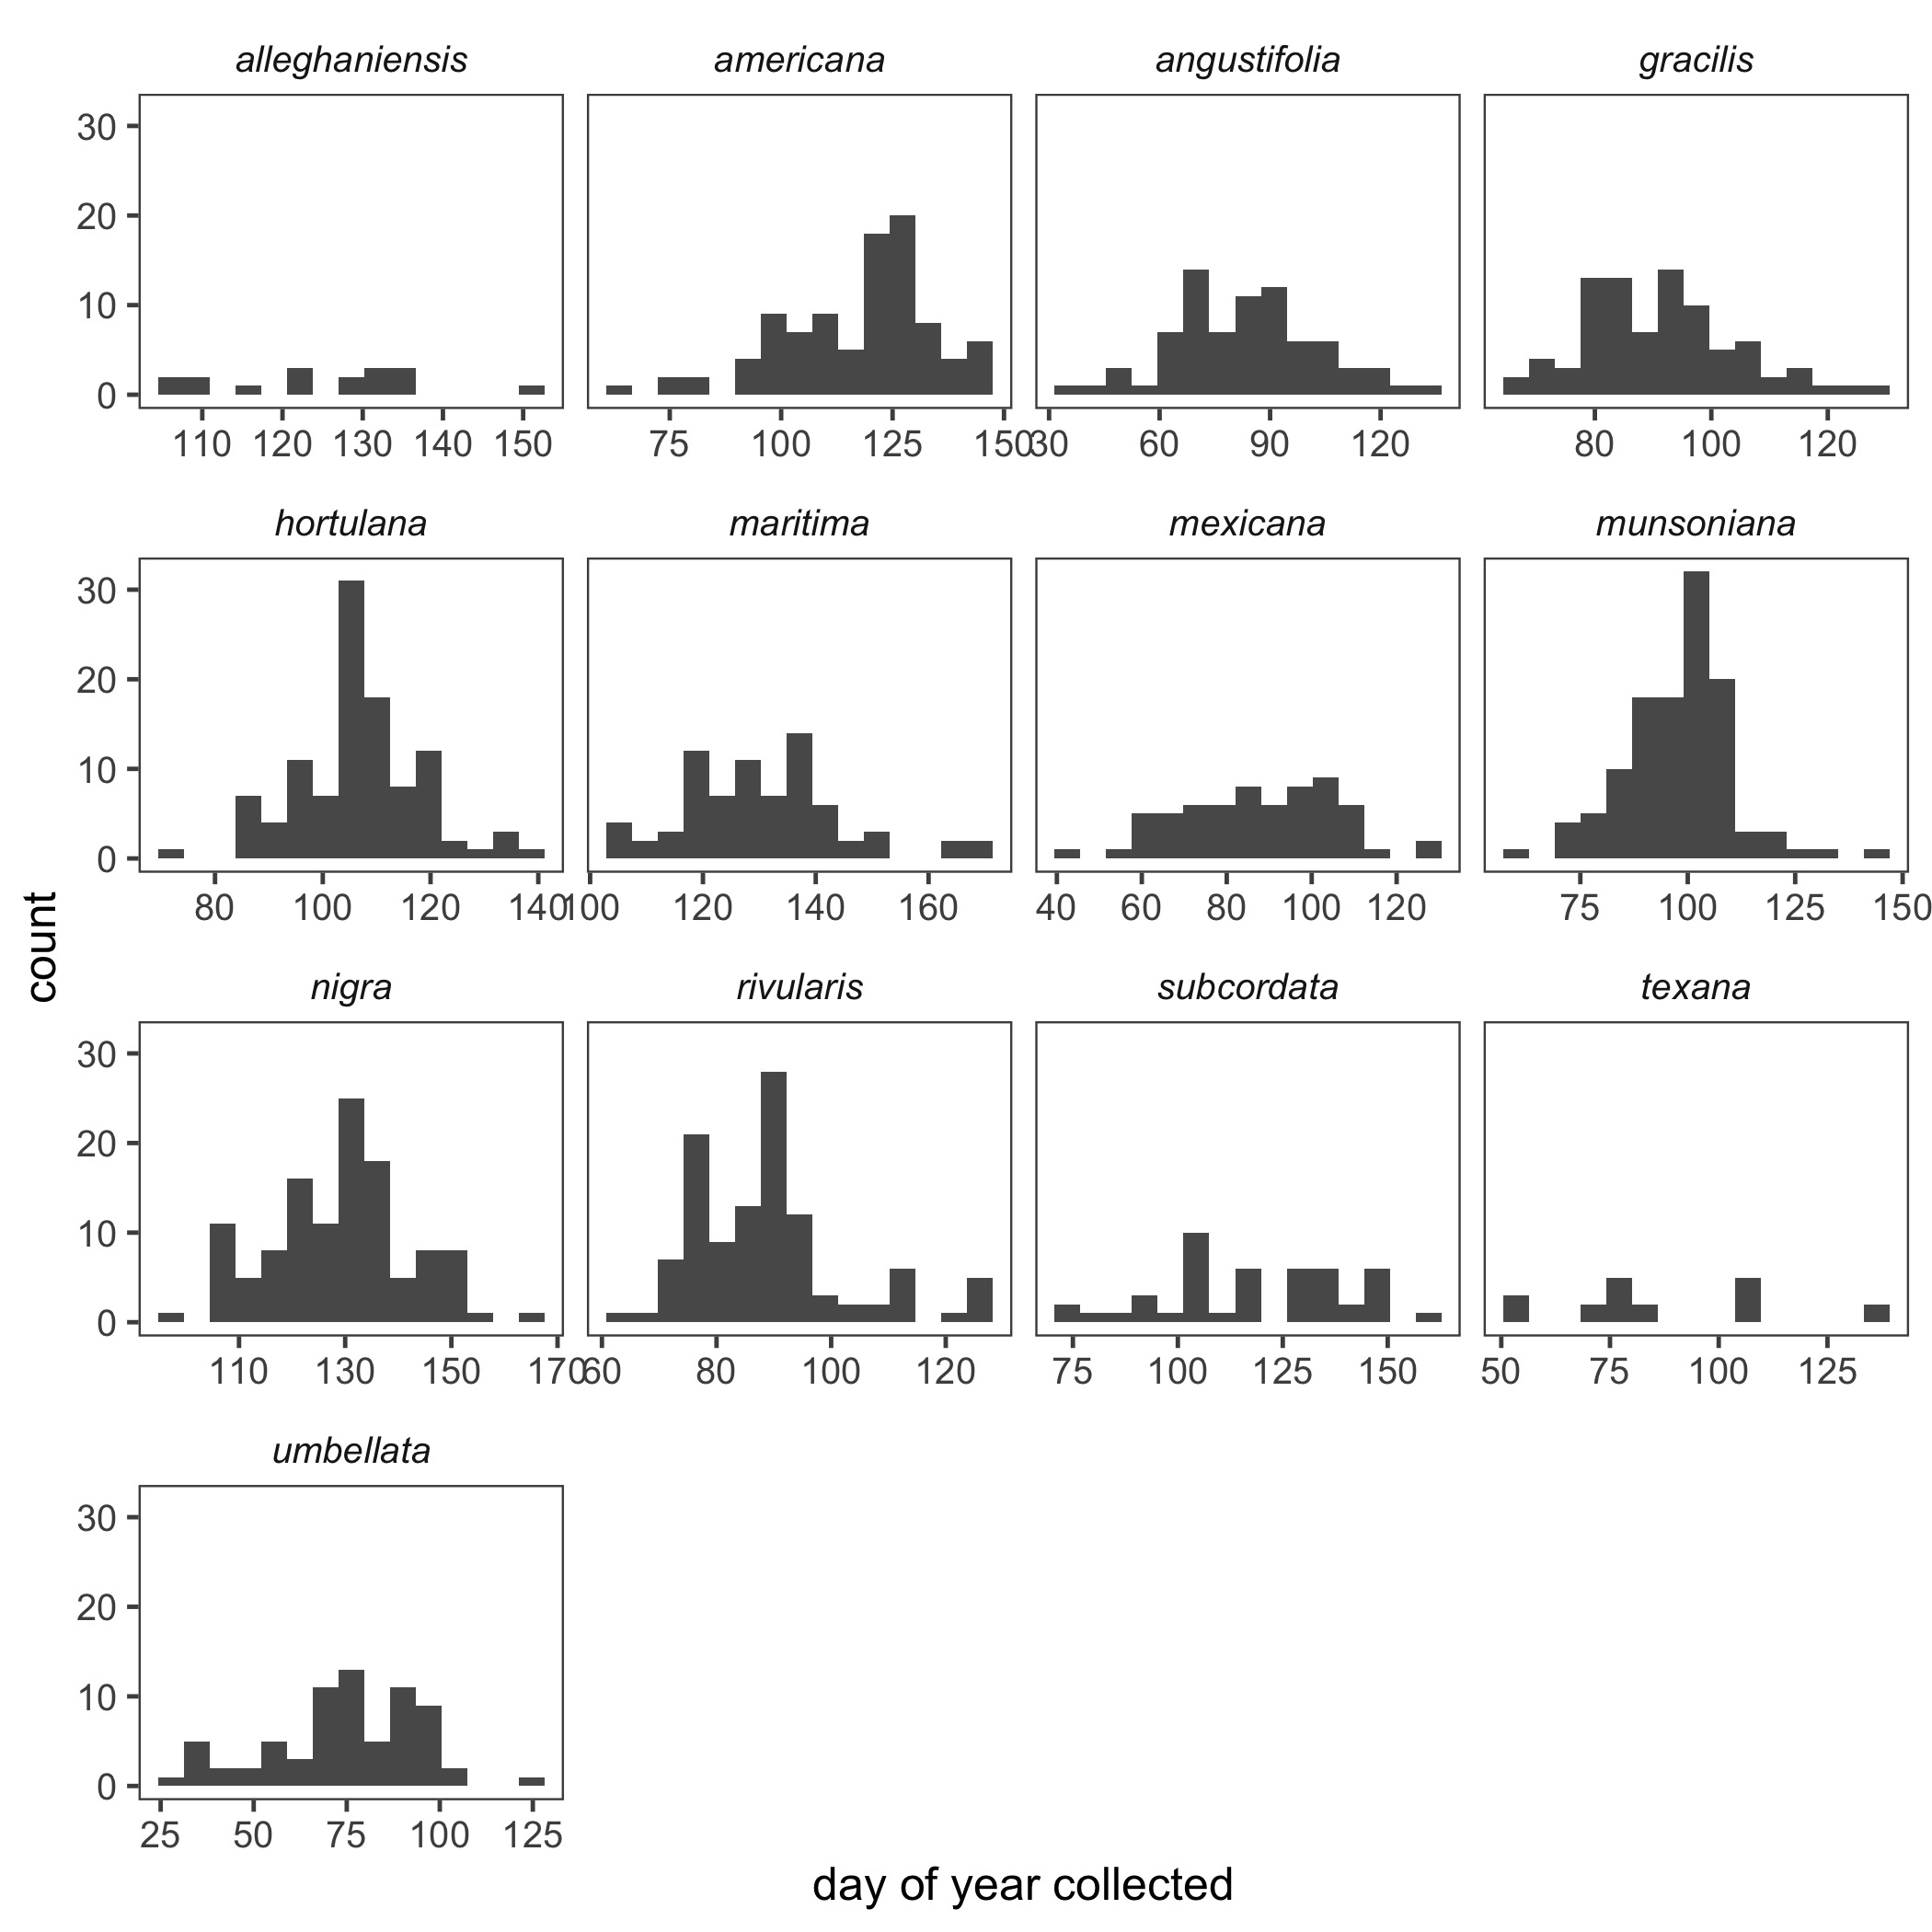
\includegraphics[width=.95\textwidth]{..//..//Plots/whatReviwerswant/seasonal_distrbn.jpeg}
    \caption{Sampling is uneven}
    \label{fig:samps}
\end{figure}


\begin{figure}[h!]
    \centering
 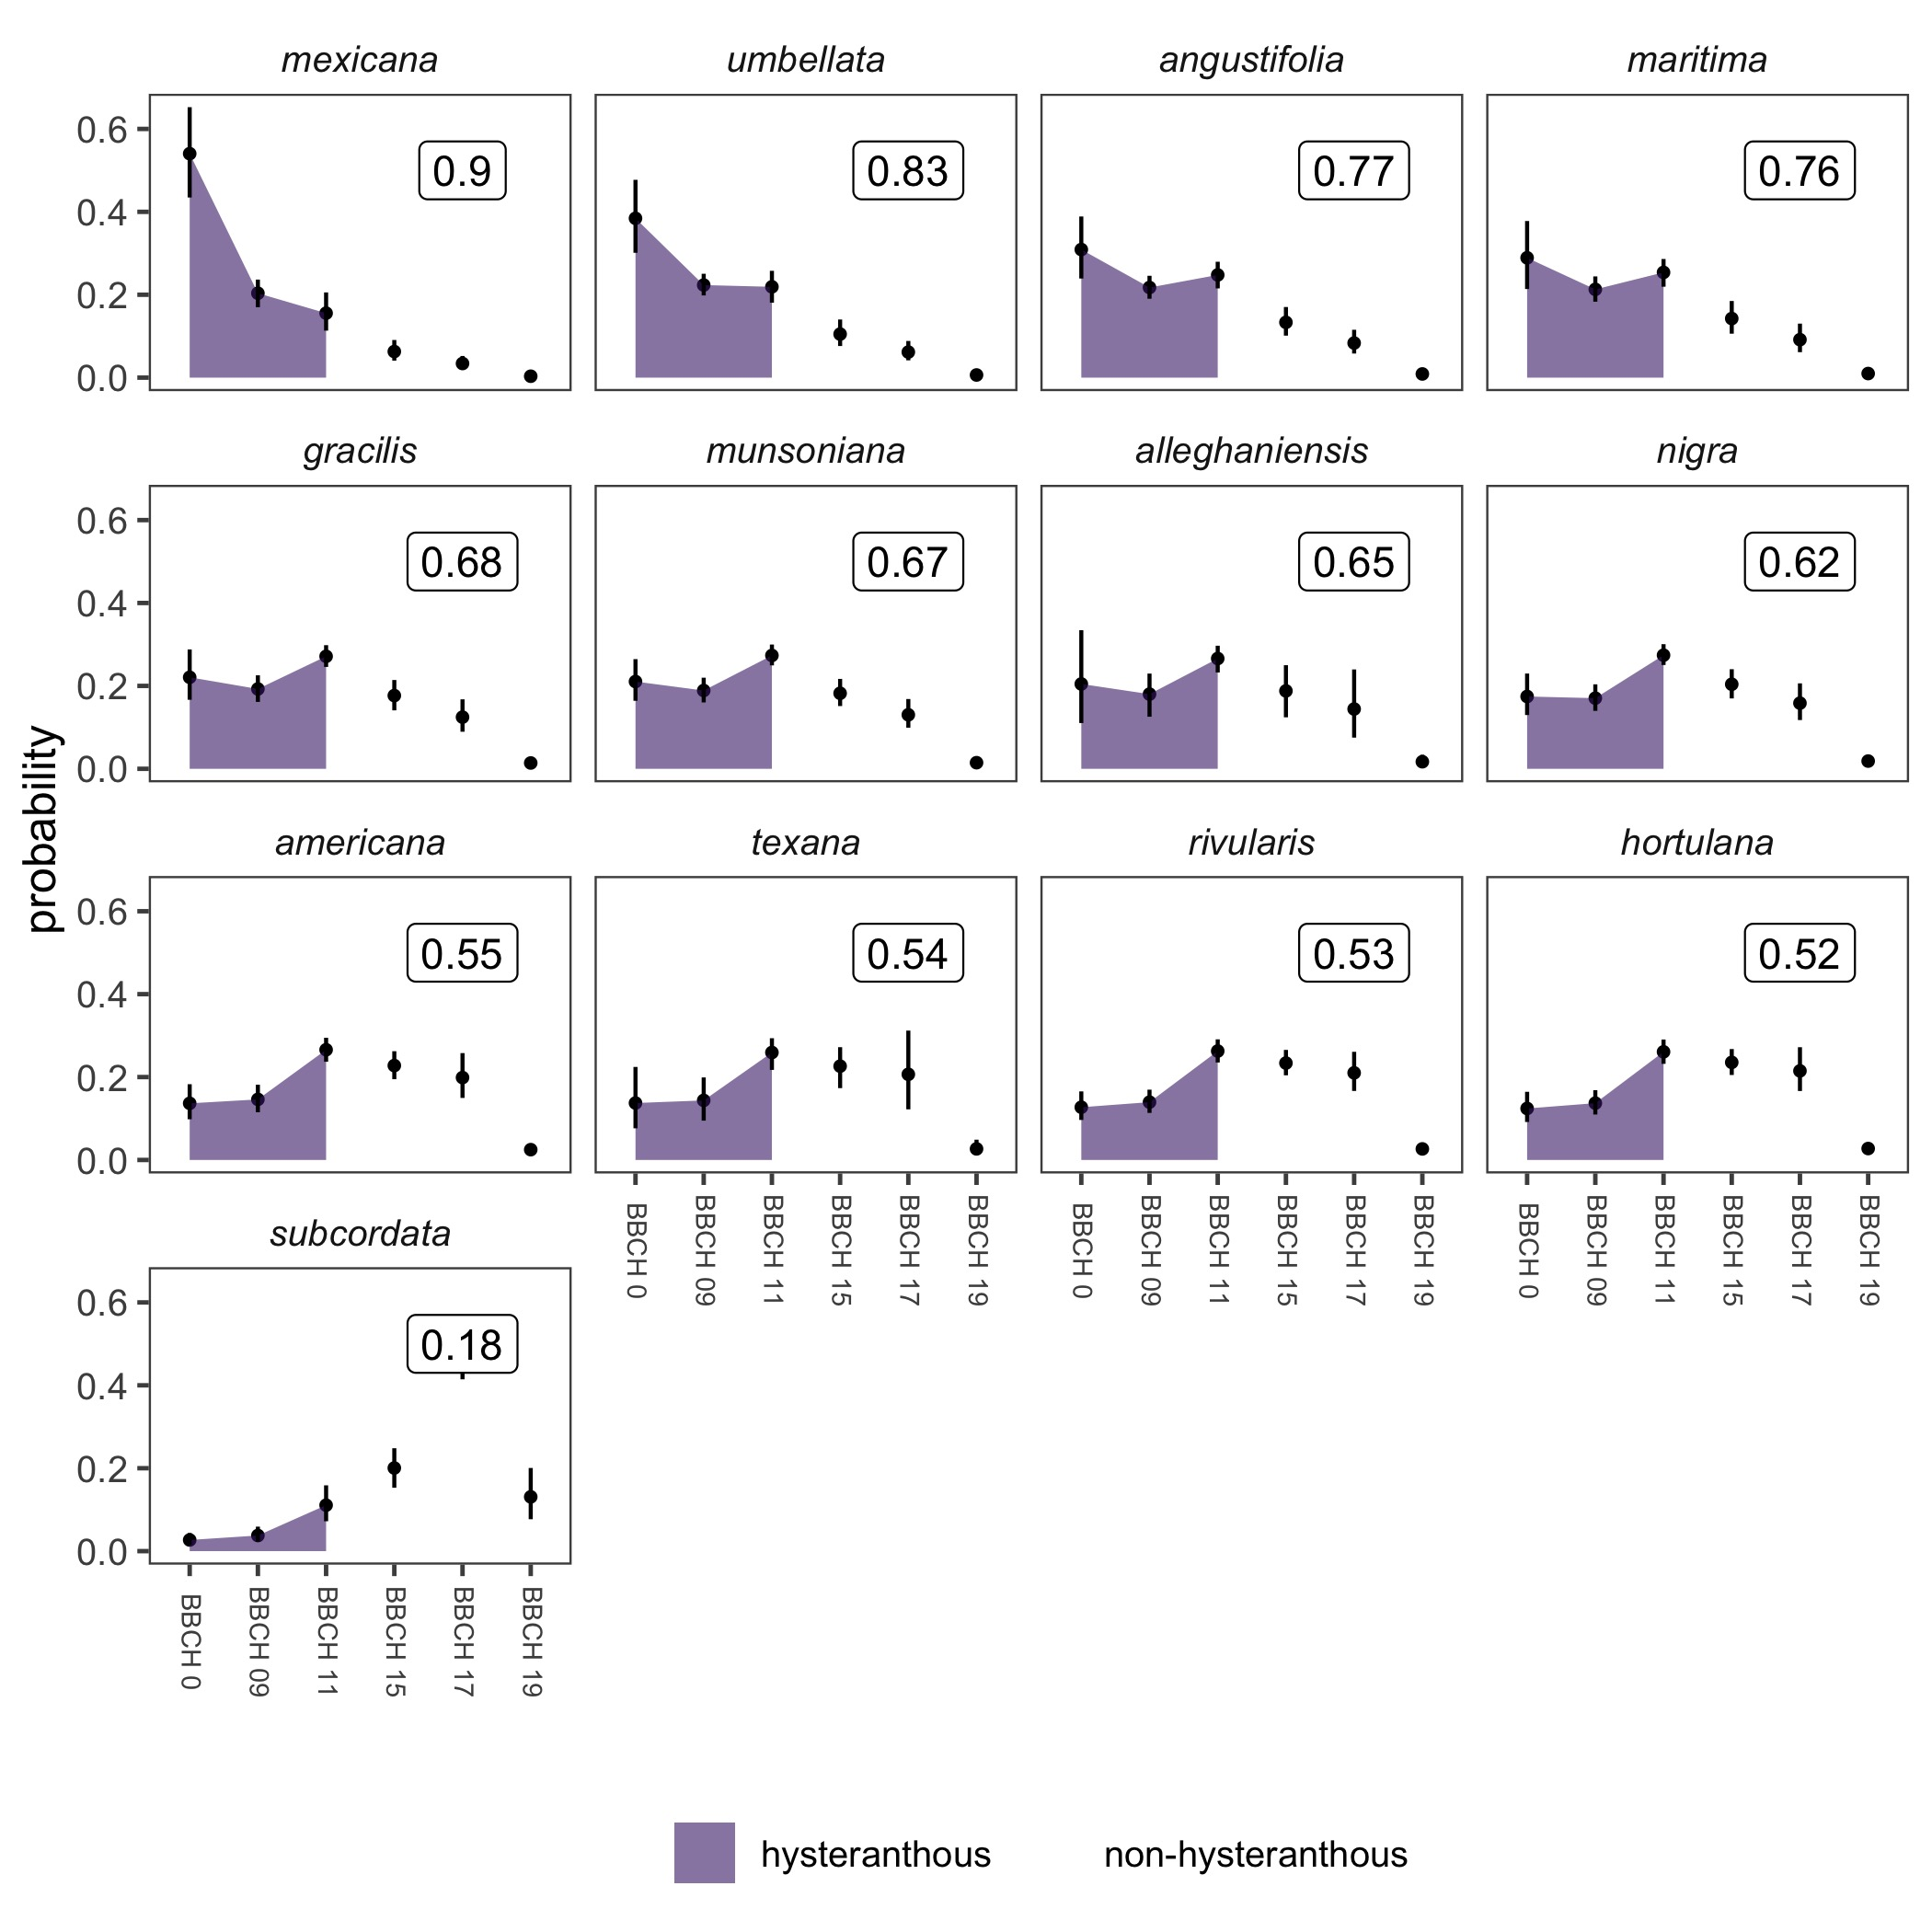
\includegraphics[width=.95\textwidth]{..//..//Plots/whatReviwerswant/sps_preds_nodoy4supp.jpeg}
    \caption{This the model predictions without doy}
    \label{fig:nodoy}
\end{figure}

\begin{figure}[h!]
    \centering
 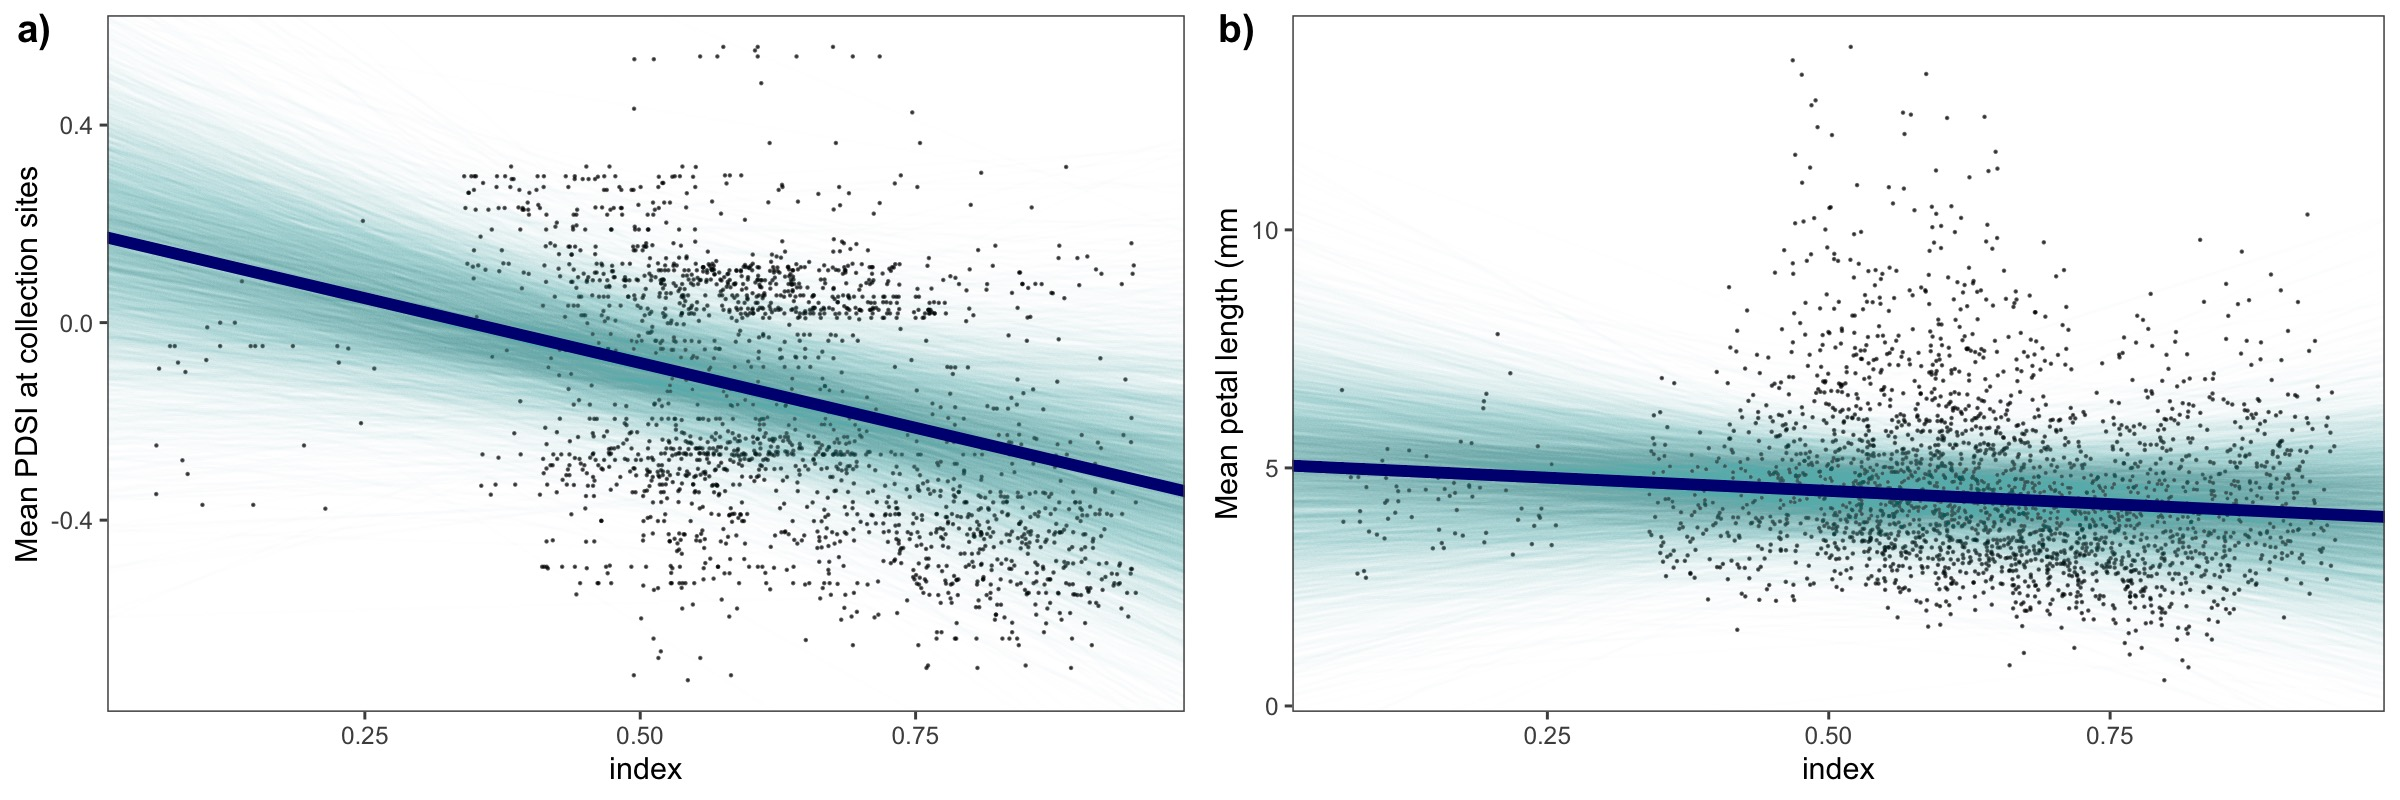
\includegraphics[width=.95\textwidth]{..//..//Plots/dataplots_SUPP.jpeg}
    \caption{This is the seperate model}
    \label{fig:seps}
\end{figure}

\end{document}
